\documentclass{beamer}

% reduce size of title
\setbeamerfont{frametitle}{size=\normalsize}

% to color fonts with \textcolor
\usepackage{color} 
    
% make a command for gray sub-items and continued subitems
\newcommand{\si}[1]{\hspace{.5cm} \textcolor{gray} {#1}\\}
\newcommand{\sicont}[1]{\hspace{1cm} \textcolor{gray} {#1}\\}

% hyperref + a generic link with purple coloring
\usepackage{hyperref}
\newcommand{\cref}[1]{\href{#1}{[\textcolor{purple}{link}]}}

% permit absolute textblock positioning
% can use showboxes option to see where textblocks are sitting
\usepackage[absolute,overlay]{textpos}

%remove navigation symbols
\setbeamertemplate{navigation symbols}{}

% for DAGs
\usepackage{tikz}
\usetikzlibrary{positioning,shapes.geometric}
% define arrows that look like the tikz versions
\newcommand*{\RightArrow}[1][]{\mathbin{\tikz [baseline=-0.25ex,-latex, #1] \draw [#1] (0pt,0.5ex) -- (1.3em,0.5ex);}}
\newcommand*{\LeftArrow}[1][]{\mathbin{\tikz [baseline=-0.25ex,-latex, #1] \draw [#1] (1.3em,0.5ex) -- (0pt,0.5ex);}}
% boxes around letters
\makeatletter
\renewcommand{\boxed}[1]{\text{\fboxsep=.2em\fbox{\m@th$\displaystyle#1$}}}
\makeatother

% for flow charts per http://www.texample.net/tikz/examples/simple-flow-chart/
\usetikzlibrary{shapes,arrows}
\tikzstyle{decision} = [diamond, draw, fill=blue!20, 
    text width=4.5em, text badly centered, node distance=3cm, inner sep=0pt]
\tikzstyle{block} = [rectangle, draw, fill=blue!20, 
    text width=5em, text centered, rounded corners, minimum height=4em]
\tikzstyle{line} = [draw, -latex']
\tikzstyle{cloud} = [draw, ellipse,fill=red!20, node distance=5cm,
    minimum height=2em]
    
% permit a background box
\usetikzlibrary{calc, fit} 

% shrug emoji
\newcommand{\shrug}[1][]{%
\begin{tikzpicture}[baseline,x=0.8\ht\strutbox,y=0.8\ht\strutbox,line width=0.125ex,#1]
\def\arm{(-2.5,0.95) to (-2,0.95) (-1.9,1) to (-1.5,0) (-1.35,0) to (-0.8,0)};
\draw \arm;
\draw[xscale=-1] \arm;
\def\headpart{(0.6,0) arc[start angle=-40, end angle=40,x radius=0.6,y radius=0.8]};
\draw \headpart;
\draw[xscale=-1] \headpart;
\def\eye{(-0.075,0.15) .. controls (0.02,0) .. (0.075,-0.15)};
\draw[shift={(-0.3,0.8)}] \eye;
\draw[shift={(0,0.85)}] \eye;
% draw mouth
\draw (-0.1,0.2) to [out=15,in=-100] (0.4,0.95); 
\end{tikzpicture}}

\begin{document}

%% Title Page
\begin{frame}

\begin{textblock}{13.5}[.5,.5](8,8)
\centering
\normalsize{Predictive modeling from high-throughput results}
\end{textblock}

\begin{textblock}{6}(9,12.7)
\begin{flushright}
\scriptsize{Travis Gerke, ScD}\\
\tiny{Director of Data Science, PCCTC}\\
\tiny{gerket@mskcc.org}\\
\includegraphics[scale=.02, trim=0 1cm 0 3.5cm, clip]{figures/Twitter_Logo_Blue.png}\tiny{\href{https://twitter.com/travisgerke}{@travisgerke}}\\
\end{flushright}
\end{textblock}

\begin{textblock}{6}(1,13.8)
\tiny{AACR IME Workshop\\July 30, 2021\\}
\end{textblock}

\begin{textblock}{6}(9,0)
\begin{flushright}
\includegraphics[width=2.2cm, trim=0 0 0 0]{figures/PCCTClogoCMYK.eps}
\end{flushright}
\end{textblock}

\begin{textblock}{2}(1,.6)
\centering
\includegraphics[scale=.02, trim=0 1cm 0 3.5cm, clip]{figures/Twitter_Logo_Blue.png}\\
\scriptsize{\#AACRMolEpi}
\end{textblock}

\end{frame}


\small{

%\begin{frame}[t]
%\frametitle{First, what do you want to find?}
%Prognostic marker: informs about outcome (independent of treatment)\\
%\si{Ex: PIK3CA mutation in HER2$^+$ BrCa predicts similarly shorter time}
%\sicont{to progression whether treated with Pertuzumab or Trastuzumab}
%\vspace{.2cm}
%Predictive marker: informs about treatment effectiveness\\
%\si{Ex: EGFR mutated NSCLC benefit more from erlotinib treatment}
%\vspace{.2cm}
%HUGE ambiguity and variation in use of the above two terms! \\
%\si{Sometimes, predictive = prediagnostic risk marker}
%\si{Or, prognostic = anything that predicts outcome (even if treated)}
%\si{Markers can be both prognostic and predictive}
%\begin{center}
%\includegraphics[scale=.6, trim=1cm 0 0 .5cm]{figures/predprog.png}
%\end{center}
%\end{frame}
%
%\begin{frame}[t]
%\frametitle{Predictive markers of treatment effectiveness}
%The previous JCO article states that a statistical treatment $\times$ marker \\
%\hspace{.5cm} interaction indicates a predictive marker\\
%\si{i.e.\ must show effect measure modification exists}
%\si{But existence of such depends on what effect measure is of interest}
%\si{Risk/odds ratios are multiplicative. Risk differences are additive.}
%\vspace{.2cm}
%Fun(?) fact: if two exposures are associated with outcome, then absence\\
%\hspace{.5cm} of a multiplicative interaction implies an additive interaction (and\\
%\hspace{.5cm} vice versa)\\
%\si{Put another way, there must be an interaction when you have two}
%\sicont{markers associated with outcome}
%\vspace{.2cm}
%So, which effect measure should you use?\\
%\si{Depends on the application: as a general rule, additive often better}
%\sicont{measures public health impact}
%\si{See VanderWeele and Knol 2014 \cref{https://cdn1.sph.harvard.edu/wp-content/uploads/sites/603/2013/03/InteractionTutorial.pdf} for details}
%\si{Many high-dimensional data analysis techniques don't account for}
%\sicont{this subtlety, so the burden is on you to make sure you're}
%\sicont{estimating the ``right'' effects!}
%\end{frame}

\begin{frame}[t]
\frametitle{What we're going to talk about}
1. Feature selection\\
\vspace{.1cm}
2. How do we know models are good?\\
\vspace{.1cm}
3. The dangers of overfitting\\
\vspace{1cm}
\begin{center}
\includegraphics[scale=.05, trim=0 0 0 0]{figures/alex-chumak-zGuBURGGmdY-unsplash.jpg}
\end{center}
\end{frame}


\begin{frame}[t]
\frametitle{One view of a high-throughput study}
You measure lots of features ($p$) in some patients ($n$) with follow-up
\begin{center}
\scalebox{.7}{
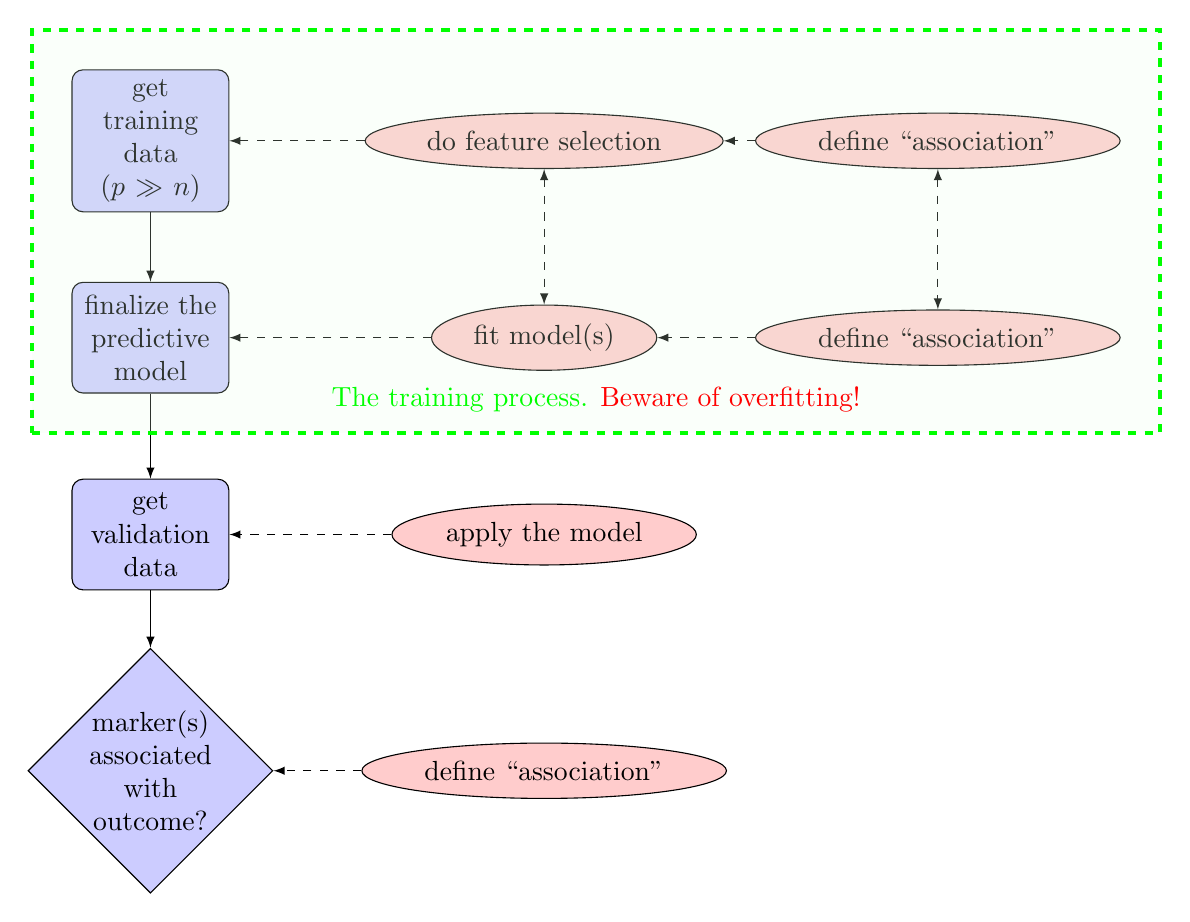
\begin{tikzpicture}[node distance = 2.5cm, auto]
    % Place nodes
    \node [block] (1l) {get training data ($p\gg n$)};
    \node [cloud, right of=1l] (1c) {do feature selection};
    \node [cloud, right of=1c] (1r) {define ``association''};
    \node [block, below of=1l] (2l) {finalize the predictive model};
    \node [cloud, right of=2l] (2c) {fit model(s)};
    \node [cloud, right of=2c] (2r) {define ``association''};    
    \node [block, below of=2l] (3l) {get validation data};
    \node [cloud, right of=3l] (3c) {apply the model};
    \node [decision, below of=3l] (4l) {marker(s) associated with outcome?};    
    \node [cloud, right of=4l] (4c) {define ``association''};    
%    % Draw edges
    \path [line, ->, >=latex] (1l) -- (2l);
    \path [line, ->, >=latex] (2l) -- (3l);
    \path [line, ->, >=latex] (3l) -- (4l);    
    \path [line,dashed, ->, >=latex] (1c) -- (1l);
    \path [line,dashed, ->, >=latex] (1r) -- (1c);
    \path [line,dashed, ->, >=latex] (2c) -- (2l);   
    \path [line,dashed, ->, >=latex] (2r) -- (2c);
    \path [line,dashed,<->, >=latex] (1r) -- (2r);
    \path [line,dashed,<->,>=latex] (1c) -- (2c);
    \path [line,dashed, ->, >=latex] (3c) -- (3l);   
    \path [line,dashed, ->, >=latex] (4c) -- (4l);       
      % background box
    \node (X) [draw=green, fit= (1l) (1c) (1r) (2l) (2c) (2r),  inner sep=0.50cm, 
            dashed, ultra thick, fill=green!10, fill opacity=0.2] {}; 
     \node [yshift=3.0ex, green] at (X.south) {The training process. \textcolor{red}{Beware of overfitting!}};     
\end{tikzpicture}
}
\end{center}
\end{frame}

\begin{frame}[t]
\frametitle{Feature selection}
Typical scenario: You've measured thousands of genes/SNPs/markers\\
\hspace{.5cm} and need to know which ones are important\\
\si{You probably also have some clinical variables too}
\vspace{.2cm}
Your criteria for including variables in your model depends on the goal\\
\si{Causal determinants/intervention targets: choose with expert input}
\si{Risk prediction (prognostication): choose whatever works}
\vspace{.2cm}
So, for prediction, fear not the confounded relationship!\\
\begin{center}
\includegraphics[scale=.25, trim=0cm 0cm 0cm .95cm, clip]{figures/icrecream.png}
\end{center}
\end{frame}

\begin{frame}[t]
\frametitle{Feature selection: abbreviated list of methods}
Exhaustive search: pick best model from all variable combinations\\
\si{Becomes computationally awful; 30 variables $\implies 1.1$ trillion models}
\vspace{.2cm}
Greedy search: in a stepwise fashion, pick the next best variable(s)\\
\si{Forward and backward selection are examples of this method}
\si{Faster, but with the tradeoff that you might not find the best set}
\vspace{.2cm}
Penalized regression such as lasso or elastic net\\
\si{Convenient to think of these as fancy greedy algorithms}
\si{Fast, easy to interpret}
\vspace{.2cm}
Variable importance measures from ensemble methods\\
\si{Example: random forests consist of many classification trees, where}
\sicont{each tree ``votes'' for the outcome. One can assess which}
\sicont{variables were critical for accuracy in many trees.}
\vspace{.2cm}
Information-based filtering (only unsupervised method on this page)\\
\si{Examples: Remove all features correlated at $>0.70$; PCA filtering}
\si{This does not select based on how well outcome is predicted!}
\vspace{.2cm}
Heuristic: choose your own adventure!\\
\si{Make your own rules. If it validates in independent data, you win.}
\end{frame}

\begin{frame}[t]
\frametitle{Feature selection: inference in training}
Note that $p$-value thresholds were not mentioned on the previous slide\\
\si{But this is not the way GWAS studies work right? (think $10^{-8}$)}
\si{Interestingly, methods for expression studies have evolved differently,}
\sicont{particularly in that there is no standard cutoff}
\si{But both types of studies have the goal of independent validation}
\vspace{.2cm}
Exercise: You're doing the first ever GWAS. When will you use $p$-values\\
\hspace{.5cm} (training, validation, neither), and what cutoffs will you use?\\
\si{Recent controversial motivation below \cref{https://simplystatistics.org/2017/06/20/lowering-the-gwas-threshold-would-save-millions-of-dollars/}}
\begin{center}
\includegraphics[scale=.25, trim=0cm 0cm 0cm .5cm]{figures/rafa.png}
\end{center}
\end{frame}

\begin{frame}[t]
\frametitle{Feature selection: opinionated list of tools}
Awesome: R/Bioconductor\\
\si{Suggested starting packages: \href{https://topepo.github.io/caret/}{\textcolor{purple}{\ttfamily{caret}}}/\href{https://tidymodels.github.io/parsnip/}{\textcolor{purple}{\ttfamily{parsnip}}}, 
\href{https://cran.r-project.org/web/packages/glmnet/index.html}{\textcolor{purple}{\ttfamily{glmnet}}}, 
\href{https://cran.r-project.org/web/packages/pamr/index.html}{\textcolor{purple}{\ttfamily{pamr}}}, 
\href{https://cran.r-project.org/web/packages/RWeka/index.html}{\textcolor{purple}{\ttfamily{RWeka}}}}
\si{For deep learning: \href{https://keras.rstudio.com/}{\textcolor{purple}{\ttfamily{Keras}}}}
\si{Stepwise selection available through the \ttfamily{step()} function}
\si{An easy language in which to write your own algorithms}
\si{Massive benefit to having bioinformatics packages for iterative QC}
\vspace{.2cm}
Awesome: Python, often through \href{http://scikit-learn.org/stable/index.html}{\textcolor{purple}{\ttfamily{scikit-learn}}}\\
\si{Can be a bit harder to install/maintain than R/RStudio}
\si{Note: {\ttfamily{scikit-learn}} is amazing for ML, but may provide}
\sicont{unexpected statistical inference in some specific settings \cref{https://www.reddit.com/r/statistics/comments/8de54s/is_r_better_than_python_at_anything_i_started/dxmnaef/}}
\vspace{.2cm}
Less awesome: Stata is somewhere in the middle\\
\si{Some modules exist: \href{http://econpapers.repec.org/software/bocbocode/s457932.htm}{\textcolor{purple}{\ttfamily{CHAIDFOREST}}}, 
\href{https://ideas.repec.org/c/boc/bocode/s456860.html}{\textcolor{purple}{\ttfamily{LARS}}}, and
\href{http://econpapers.repec.org/software/bocbocode/s458337.htm}{\textcolor{purple}{\ttfamily{ELTMLE}}}}
\si{Interestingly, some of those modules rely on R \shrug}
\vspace{.2cm}
Less awesome: SAS is more limiting, but it can be done\\
\si{Standard SAS can do forward/backward selection in standard models}
\si{Need Enterprise Miner for random forest, penalized regression, PCA}
\end{frame}

\begin{frame}[t]
\frametitle{Feature selection: what to do with clinicopathologic factors?}
Assuming you're not the lead biostatistician on the project, a cursory\\
\hspace{.5cm} familiarity with the methods/tools slides will likely suffice!\\
\si{How you treat known predictive factors in your study will, however,}
\sicont{be critical; and this is not a solely statistical concern}
\vspace{.2cm}
Exercise: tumor grade is highly predictive of eventual PrCa metastasis.\\
\hspace{.5cm} You profiled tumor tissue to find a gene expression signature to\\
\hspace{.5cm} predict metastasis. What do you do with the variable ``grade''?\\
\si{Bonus: what are ``confounders'' in predictive models?}
\begin{center}
\includegraphics[scale=.4, trim=0cm 0cm 0cm .5cm]{figures/confounders.png}
\end{center}
\end{frame}

\begin{frame}[t]
\frametitle{Model fit: How do we measure ``good'?}
For binary markers, we have some standard metrics\\
\si{Sensitivity: $se=P(M^+\mid D^+)$; specificity: $sp=P(M^-\mid D^-)$}
\si{Positive predictive value: $PPV=P(D^+\mid M^+)$}
\si{Negative predictive value: $NPV=P(D^-\mid M^-)$}
\vspace{.2cm}
But risk exists on a continuum $\implies$ probabilistic classifiers\\
\si{Evaluating prediction accuracy more difficult when we can't fit}
\sicont{results into a $2\times 2$ table}
\begin{center}
\includegraphics[scale=.45, trim=0cm 0cm 0cm 0cm]{figures/predmodel.png}
\end{center}
\end{frame}

%\begin{frame}[t]
%\frametitle{Measures of overall performance/calibration}
%Want minimal distance between predicted outcome and actual outcome\\
%\si{For continuous outcomes, the familiar residual $Y-\hat Y$}
%\si{These residuals can help estimate variance explained ($R^2$)}
%\si{For binary outcomes, we have a $Y\in\{0,1\}$ and $\hat Y=\hat p$}
%\si{Extending $R^2$ for binary outcomes: Nagelkerke's $R^2$ and Brier score}
%\si{Can also look at goodness-of-fit such as BIC/AIC, Hosmer-Lemeshow}
%\si{Calibration: Among 100 patients with 20\% predicted risk, 20/100}
%\sicont{patients should be a case}
%\begin{center}
%\includegraphics[scale=.22, trim=0cm 0cm 0cm 1cm]{figures/calibplot.pdf}%%%need to make validation graph
%\end{center}
%\end{frame}

\begin{frame}[t]
\frametitle{Model fit: Discrimination}
How well the model separates cases from non-cases\\
\si{Distinct from prediction accuracy: could predict all cases with}
\sicont{$\hat p=0.51$ and non-cases with $\hat p=0.50$ for perfect discrimination}
\vspace{.2cm}
The most common statistic: area under the ROC curve (AUC)\\
\si{The probability that a randomly selected case will have a higher}
\sicont{predicted risk than a randomly selected non-case}
\begin{center}
\includegraphics[scale=.32, trim=0cm 0cm 0cm .2cm]{figures/aucEx.pdf}
\end{center}
 \end{frame}

\begin{frame}[t]
\frametitle{Model fit: Measures related to clinical utility}
Most of the above measures assume the ``cost'' of a false negative is the\\
\hspace{.5cm} same as that of a false positive\\
\si{In practice, this is most often not the case!}
\vspace{.2cm}
Reclassification: how does a new marker shift predicted classifications?\\
\vspace{.2cm}
Decision curve analysis: visualize/test the benefit of competing models\\
\vspace{.2cm}
Partial area under the ROC curve (pAUC): only calculate AUC for areas\\
\hspace{.5cm} clinically applicable\\
\begin{center}
\includegraphics[scale=.27, trim=2.4cm 0cm 0cm .5cm]{figures/paucEx2.pdf}
\end{center}
\end{frame}

%\begin{frame}[t]
%\frametitle{An important note about testing for improvement}
%Measures like AUC notoriously suffer from low power when looking at\\
%\hspace{.5cm} new markers\\
%\si{Turns out, all you need to do is test your new marker in an ordinary}
%\sicont{regression that controls for existing markers}
%\si{This is a very powerful reminder to look at simple associations}
%\sicont{(boxplots, odds ratios, etc) before/after jumping to}
%\sicont{uber-complicated methodology!}
%\begin{center}
%\includegraphics[scale=.39, trim=0cm 0cm 0cm 0cm]{figures/testing.png}
%\end{center}
%\end{frame}
%
%\begin{frame}[t]
%\frametitle{Matching your method to your objective}
%Most feature selection/model building algorithms will not directly\\
%\hspace{.5cm} maximize something like AUC (or whatever your objective is)\\
%\si{They often maximize a likelihood (and, hence, overall performance)}
%\si{Don't worry too much: often there is overlap in what ``good'' means}
%\si{Nonetheless, it's an active area of research}
%\begin{center}
%\includegraphics[scale=.33, trim=0cm 0cm 0cm 1cm]{figures/google.png}
%\end{center}
%\end{frame}

\begin{frame}[t]
\frametitle{The dangers of overfitting: cross-validation}
When you have $p>n$, you can \emph{always} find a perfect model\\
\si{But this model is extremely unlikely to work in other data}
\si{If you do this, you have overfit your data}
\vspace{.2cm}
One strategy to guard against overfitting: cross-validation\\
\si{If possible, nest \emph{everything} you do in the training data in the}
\sicont{cross-validation step}
%http://blog.kaggle.com/2015/06/29/scikit-learn-video-7-optimizing-your-model-with-cross-validation/
\begin{center}
\includegraphics[scale=.28, trim=0cm 0cm 0cm 1cm]{figures/cv.png}
\end{center}
\end{frame}

\begin{frame}[t]
\frametitle{The dangers of overfitting: external validation}
Even if you use cross-validation, you may have still overfit and selected\\
\hspace{.5cm} noisy features of your training data\\
\si{External validation in an independent data source is \emph{critical}!}
\si{If this is impossible (e.g.\ due to cost), you can sometimes hold out a}
\sicont{portion of your initial data until the very end, though this is not}
\sicont{as powerful}
\begin{center}
\includegraphics[scale=.39, trim=0cm 0cm 0cm 0cm]{figures/validation.png}
\end{center}
\end{frame}

\begin{frame}[t]
\frametitle{The dangers of overfitting: model complexity}
There is generally a ``sweet spot'' for model complexity with respect to\\
\hspace{.5cm} ultimate performance in test (external) data\\
\si{Cross-validation can help find this sweet spot, but is not a panacea}
\si{Often the best case is small number of features with strong signal}
\begin{center}
\includegraphics[scale=.5, trim=0cm 0cm 0cm 0cm]{figures/complexity.png}
\end{center}
\begin{flushright}
\tiny{$^*$ Figure from Hastie et al. \emph{Elements of Statistical Learning}}
\end{flushright}
\end{frame}


\begin{frame}[t]
\frametitle{Exercise}
You have measured expression of 6000 genes from prostate tumors at diagnosis and have 30 years of follow-up data. You would like to build a prediction model for risk of future metastasis. Which of the following strategies would you use?\\
\si{Established clinical parameters (e.g.\ Gleason grade and stage) alone}
\si{Clinical parameters + top 10 genes from logistic regression}
\si{Clinical parameters + machine learning algorithm using all genes}
\vspace{.2cm}
Important to consider: which is most likely to validate in independent data, and which has the highest risk of overfitting?
\end{frame}

\begin{frame}[t]
\frametitle{Exercise}
\begin{center}
\includegraphics[scale=.5, trim=0cm 0cm 0cm 0cm]{figures/sboner.png}
\end{center}
\end{frame}

%\begin{frame}[t]
%\frametitle{Exercise}
%Whole-transcriptome tumor expression at surgery and follow-up data for recurrence exists in 5 independent academic centers. How will you combine/separate this data to train and validate a prediction model?\\
%\si{Some options follow (however, feel free to propose another)}
%\si{Pool all of the data then randomly create 5 equally-sized cohorts.}
%\sicont{Train a model in 4 of these, test performance in the last.}
%\si{Train a model in pooled data from 4 of the original cohorts. Test}
%\sicont{performance in the last.}
%\si{Train a model in data from 1 of the original cohorts. Test}
%\sicont{performance in pooled data from the 4 remaining cohorts.}
%\end{frame}
}
\end{document}